% -*- mode: Latex; fill-column: 120; -*-
\documentclass{article}\usepackage[]{graphicx}\usepackage[]{color}
%% maxwidth is the original width if it is less than linewidth
%% otherwise use linewidth (to make sure the graphics do not exceed the margin)
\makeatletter
\def\maxwidth{ %
  \ifdim\Gin@nat@width>\linewidth
    \linewidth
  \else
    \Gin@nat@width
  \fi
}
\makeatother

\definecolor{fgcolor}{rgb}{0.345, 0.345, 0.345}
\newcommand{\hlnum}[1]{\textcolor[rgb]{0.686,0.059,0.569}{#1}}%
\newcommand{\hlstr}[1]{\textcolor[rgb]{0.192,0.494,0.8}{#1}}%
\newcommand{\hlcom}[1]{\textcolor[rgb]{0.678,0.584,0.686}{\textit{#1}}}%
\newcommand{\hlopt}[1]{\textcolor[rgb]{0,0,0}{#1}}%
\newcommand{\hlstd}[1]{\textcolor[rgb]{0.345,0.345,0.345}{#1}}%
\newcommand{\hlkwa}[1]{\textcolor[rgb]{0.161,0.373,0.58}{\textbf{#1}}}%
\newcommand{\hlkwb}[1]{\textcolor[rgb]{0.69,0.353,0.396}{#1}}%
\newcommand{\hlkwc}[1]{\textcolor[rgb]{0.333,0.667,0.333}{#1}}%
\newcommand{\hlkwd}[1]{\textcolor[rgb]{0.737,0.353,0.396}{\textbf{#1}}}%
\let\hlipl\hlkwb

\usepackage{framed}
\makeatletter
\newenvironment{kframe}{%
 \def\at@end@of@kframe{}%
 \ifinner\ifhmode%
  \def\at@end@of@kframe{\end{minipage}}%
  \begin{minipage}{\columnwidth}%
 \fi\fi%
 \def\FrameCommand##1{\hskip\@totalleftmargin \hskip-\fboxsep
 \colorbox{shadecolor}{##1}\hskip-\fboxsep
     % There is no \\@totalrightmargin, so:
     \hskip-\linewidth \hskip-\@totalleftmargin \hskip\columnwidth}%
 \MakeFramed {\advance\hsize-\width
   \@totalleftmargin\z@ \linewidth\hsize
   \@setminipage}}%
 {\par\unskip\endMakeFramed%
 \at@end@of@kframe}
\makeatother

\definecolor{shadecolor}{rgb}{.97, .97, .97}
\definecolor{messagecolor}{rgb}{0, 0, 0}
\definecolor{warningcolor}{rgb}{1, 0, 1}
\definecolor{errorcolor}{rgb}{1, 0, 0}
\newenvironment{knitrout}{}{} % an empty environment to be redefined in TeX

\usepackage{alltt}

\usepackage[letterpaper,margin=1in]{geometry}
\usepackage[breaklinks=true,colorlinks=true,urlcolor=blue]{hyperref}
\usepackage{bookmark}
\usepackage{times}
\usepackage{amsmath}
%\usepackage{graphicx}\usepackage[]{color}  knitr adds these
\IfFileExists{upquote.sty}{\usepackage{upquote}}{}
\begin{document}
\title{FigS9: Desert Length Distribution Boxplot for ``Supplement''}
\maketitle

\tableofcontents

\section{Intro}
A simple driver script to build above fig.  

\section{Preliminaries}
Load utility R code and do setup:

\begin{knitrout}\footnotesize
\definecolor{shadecolor}{rgb}{0.969, 0.969, 0.969}\color{fgcolor}\begin{kframe}
\begin{alltt}
\hlkwd{source}\hlstd{(}\hlstr{'../../../R/wlr.R'}\hlstd{)} \hlcom{# load util code; path relative this folder or sibling in scripts/larrys }
\end{alltt}
\begin{verbatim}
## Running as: ruzzo @ macreg15026.dyn.cs.washington.edu; SVN Id, I miss you.  $Id: wlr.R  2017-07-21 or later $
\end{verbatim}
\begin{alltt}
\hlkwd{setup.my.wd}\hlstd{(}\hlstr{'paperfigs'}\hlstd{)}   \hlcom{# set working dir; UPDATE if this file moves, or if COPY/PASTE to new file}
\hlkwd{setup.my.knitr}\hlstd{(}\hlstr{'FigS9-desert-len-boxplot-knitr/'}\hlstd{)} \hlcom{# knitr's "unnamed-chunk-nnn" figures}
\hlstd{my.figs.dir} \hlkwb{<-} \hlstr{'FigS9-desert-len-boxplot-figs-mine/'}  \hlcom{# my named figures}
\hlkwd{generic.setup}\hlstd{(my.figs.dir)}
\end{alltt}
\end{kframe}
\end{knitrout}
\begin{knitrout}\footnotesize
\definecolor{shadecolor}{rgb}{0.969, 0.969, 0.969}\color{fgcolor}\begin{kframe}
\begin{alltt}
\hlcom{# from svn+ssh://ceg1.ocean.washington.edu/var/svn/7_strains/trunk/code/snpNB/data}
\hlkwd{load}\hlstd{(}\hlstr{'../../../data/des.rda'}\hlstd{)} \hlcom{# defines "des"}
\hlstd{des.df} \hlkwb{<-} \hlkwd{des.to.df}\hlstd{(des)}      \hlcom{# convert to data.frame}
\end{alltt}
\end{kframe}
\end{knitrout}

\section{The Fig}

\begin{knitrout}\footnotesize
\definecolor{shadecolor}{rgb}{0.969, 0.969, 0.969}\color{fgcolor}\begin{kframe}
\begin{alltt}
\hlkwd{pdf}\hlstd{(}\hlkwd{paste}\hlstd{(my.figs.dir,} \hlstr{'FigS9-desert-len-boxplot-fig.pdf'}\hlstd{,} \hlkwc{sep}\hlstd{=}\hlstr{''}\hlstd{),}\hlkwc{width}\hlstd{=}\hlnum{6.5}\hlstd{,}\hlkwc{height}\hlstd{=}\hlnum{5}\hlstd{)}
\hlkwd{boxplot}\hlstd{(des.df[[}\hlnum{1}\hlstd{]]}\hlopt{$}\hlstd{Length}\hlopt{/}\hlnum{1000}\hlstd{,}
        \hlstd{des.df[[}\hlnum{2}\hlstd{]]}\hlopt{$}\hlstd{Length}\hlopt{/}\hlnum{1000}\hlstd{,}
        \hlstd{des.df[[}\hlnum{3}\hlstd{]]}\hlopt{$}\hlstd{Length}\hlopt{/}\hlnum{1000}\hlstd{,}
        \hlstd{des.df[[}\hlnum{4}\hlstd{]]}\hlopt{$}\hlstd{Length}\hlopt{/}\hlnum{1000}\hlstd{,}
        \hlstd{des.df[[}\hlnum{5}\hlstd{]]}\hlopt{$}\hlstd{Length}\hlopt{/}\hlnum{1000}\hlstd{,}
        \hlstd{des.df[[}\hlnum{6}\hlstd{]]}\hlopt{$}\hlstd{Length}\hlopt{/}\hlnum{1000}\hlstd{,}
        \hlstd{des.df[[}\hlnum{7}\hlstd{]]}\hlopt{$}\hlstd{Length}\hlopt{/}\hlnum{1000}\hlstd{,}
        \hlkwc{main}\hlstd{=}\hlstr{'Desert Length Distribution'}\hlstd{,}
        \hlkwc{xlab}\hlstd{=}\hlstr{'Isolate CCMP ID (Location)'}\hlstd{,}
        \hlkwc{ylab}\hlstd{=}\hlstr{'Desert Length (Kb)'}\hlstd{,}
        \hlkwc{ylim}\hlstd{=}\hlkwd{c}\hlstd{(}\hlnum{1.6}\hlstd{,}\hlnum{450}\hlstd{),}
        \hlkwc{col}\hlstd{=}\hlstr{'lightblue'}\hlstd{,}
        \hlkwc{log}\hlstd{=}\hlstr{'y'}\hlstd{)}
\hlstd{ccmp}  \hlkwb{<-} \hlkwd{substr}\hlstd{(}\hlkwd{st.locs}\hlstd{(}\hlnum{1}\hlopt{:}\hlnum{7}\hlstd{,}\hlkwc{loc}\hlstd{=F),}\hlnum{5}\hlstd{,}\hlnum{8}\hlstd{)}
\hlstd{where} \hlkwb{<-} \hlkwd{paste}\hlstd{(}\hlstr{'('}\hlstd{,}\hlkwd{st.locs}\hlstd{(}\hlnum{1}\hlopt{:}\hlnum{7}\hlstd{,}\hlkwc{id}\hlstd{=F,}\hlkwc{loc}\hlstd{=F,}\hlkwc{locabbrv}\hlstd{=T),}\hlstr{')'}\hlstd{,}\hlkwc{sep}\hlstd{=}\hlstr{''}\hlstd{)}
\hlkwd{mtext}\hlstd{(ccmp,} \hlkwc{side}\hlstd{=}\hlnum{1}\hlstd{,}\hlkwc{at}\hlstd{=}\hlnum{1}\hlopt{:}\hlnum{7}\hlstd{,}\hlkwc{line}\hlstd{=}\hlnum{0.8}\hlstd{,}\hlkwc{cex}\hlstd{=}\hlnum{1.0}\hlstd{)}
\hlkwd{mtext}\hlstd{(where,}\hlkwc{side}\hlstd{=}\hlnum{1}\hlstd{,}\hlkwc{at}\hlstd{=}\hlnum{1}\hlopt{:}\hlnum{7}\hlstd{,}\hlkwc{line}\hlstd{=}\hlnum{1.7}\hlstd{,}\hlkwc{cex}\hlstd{=}\hlnum{0.8}\hlstd{)}
\hlkwd{dev.off}\hlstd{()}
\end{alltt}
\begin{verbatim}
# pdf 
#   2
\end{verbatim}
\end{kframe}
\end{knitrout}

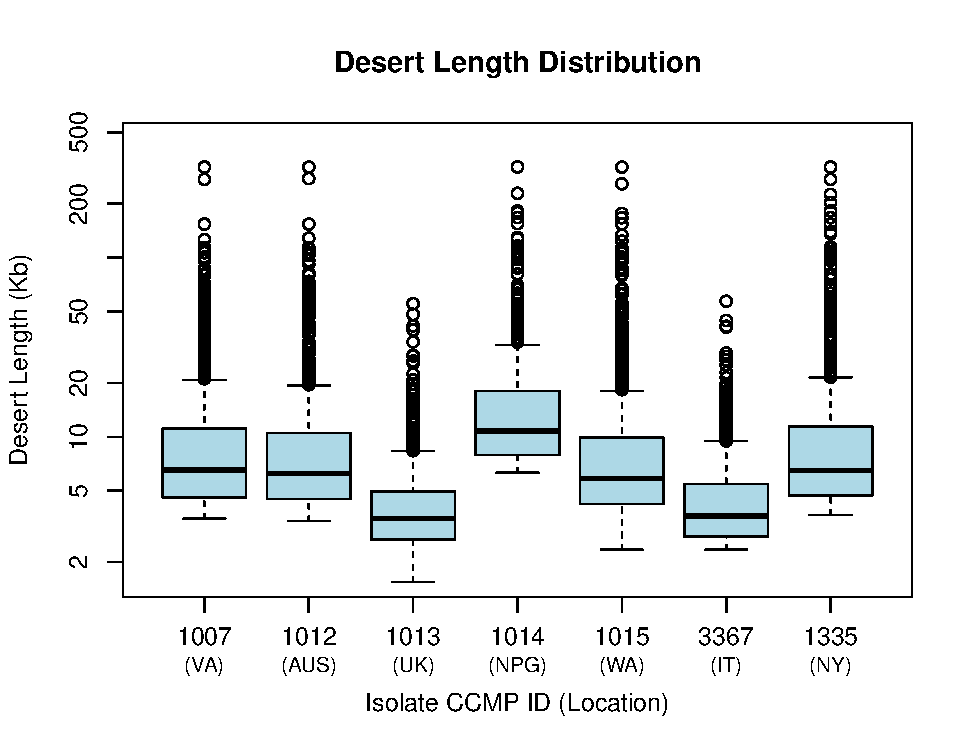
\includegraphics{FigS9-desert-len-boxplot-figs-mine/FigS9-desert-len-boxplot-fig.pdf}

\vfill\footnotesize\flushright SVN ID I miss you. $ $Id FigS9-desert-len-boxplot 2017-06-29 or later.$ $
\end{document}
